% !TEX root = main.tex

\section{计算机的运算}
\subsection{标志位}
\par 大于机器所能表示的最大正数称为上溢,小于机器所能表示的最小负数称为下溢
\begin{center}
\begin{tabular}{|c|c|c|}\hline
NF(SF) & negative & 符号\\\hline
OF(VF) & overflow & 溢出\\\hline
CF & carry & 进借位\\\hline
ZF & zero & 零\\\hline
\end{tabular}
\end{center}
\begin{itemize}
	\item 进/借位CF:\textbf{无符号数}运算结果是否超出范围,即使超出结果仍对
	\item 溢出OF:\textbf{有符号数}运算结果是否超出范围,若超出则结果不对
\end{itemize}

\subsection{位运算}
\subsubsection{左移与右移}
位运算针对二进制数,逻辑运算针对表达式的值
\begin{center}
\begin{tabular}{|c|c|c|}
\hline
\multirow{2}*{无符号数} & 逻辑左移 & 高位移出,低位补0\\
\cline{2-3} & 逻辑右移 & 低位移出,高位补0\\
\hline
\multirow{2}*{有符号数} & 算术左移 & 高位移出,低位补0\\
\cline{2-3} & 算术右移 & 低位移出,高位补\textbf{符号位}\\
\hline
\end{tabular}
\end{center}
\par 移位符号\verb'<<'和\verb'>>'不区分算术还是逻辑移位,只由参与运算的数值决定
\par 算术左移溢出判断:若移出的位不等于新的符号位,即$CF\oplus SF=1$,则溢出

\subsubsection{位扩展和位截断}
\begin{itemize}
	\item 位扩展:如\verb'float'变\verb'double';数据存入寄存器时也要扩展,\verb'lb'
	\begin{itemize}
		\item 无符号数:0扩展,即前面补0
		\item 有符号整数:符号扩展,即前面补符号
	\end{itemize}
	\item 位截断:如\verb'double'变\verb'int';强行丢弃长数的高位,可能溢出或数据不正确
\end{itemize}

\subsection{加减法}
\subsubsection{整数}
\begin{center}
\begin{tabular}{|c|c|c|}\hline
原码 & 补码 & 移码\\\hline
符号与数值单独运算 & 符号与数值一起运算 & 符号与数值一起运算\\\hline
同号相加进位溢出 & \begin{tabular}{c}变形两位补码\\01正溢出,10负溢出\end{tabular} & 两加数和和数符号都相同则溢出\\\hline
$A\pm B=A\pm B$
&$\begin{aligned}
[A+B]_c&=[A]_c+[B]_c\\
[A-B]_c&=[A]_c+[-B]_c
\end{aligned}$
&$\begin{aligned}
[A]_b+[B]_b&=[A+B]_{\textcolor{red}{c}}\\
[A]_b-[B]_b&=[A]_b+[-[B]_b]_c=[A-B]_{\textcolor{red}{c}}
\end{aligned}$\\\hline
浮点数尾数 & 定点数 & 浮点数阶码\\\hline
\end{tabular}
\end{center}
\par 注意进位和溢出的区别,在模$2^n$意义下,加负数进位相当于回到原点;而只有同号运算才可能溢出。
如$[1111-1101]_c=01111+10011=100010$,进位但不溢出(补码往前往后模特性,只有\textbf{补码}有);
而$[-1111-1101]_c=10001+10011=100100$,进位且溢出。

注意C语言是不考虑溢出的异常处理的。
\begin{itemize}
	\item unsigned整型溢出:模运算
	\item signed整型溢出:undefined behavior
	\item MIPS上的C编译器会选用无符号的算术运算指令,如\verb'addu'、\verb'addiu'、\verb'subu'
\end{itemize}

\subsubsection{浮点数}
\begin{enumerate}
	\item 对阶
	\begin{itemize}
		\item 小阶向大阶对齐,阶小尾数右移阶差$\Delta E=|E_X-E_Y|$
		\item 注意要将隐含的1移到小数部分,空出位补0
		\item 移出的低位保留到特定的附加位上
	\end{itemize}
	\item 尾数加减
	\item 结果规格化(左移或右移)
	\item 00结果不变,01舍,10强制结果为偶数,11入
	\item 判断结果正确性,是否上下溢出(当浮点数的阶码小于机器表示的最小阶码时,则下溢,将其当为0处理)
\end{enumerate}

\subsubsection{运算器件}
串行/行波进位加法器:考虑当前进位或者结合$C_{i-1}$的进位
\[\begin{aligned}
S_i&=A_i\oplus B_i\oplus C_{i-1}\\
C_i&=(A_i\oplus B_i)C_{i-1}+A_iB_i
\end{aligned}\]

并行加法器:
\begin{itemize}
	\item 若$A_iB_i=1$,则$C_{\text{out}}=1$与$C_{\text{in}}$无关(进位生成):$G_i=A_iB_i$
	\item 若$A_i+B_i=1$,则$C_{\text{out}}=1$与$C_{\text{in}}$相同(进位传递):$P_i=A_i\oplus B_i$
	\item 传递进位:$C_{i-1}P_i$
\end{itemize}

组内并行,组间串或并行(4/8位一组)
\begin{itemize}
	\item 1个SN74181构成一个4位先行进位ALU
	\item 4个SN74181串行构成一个16位单级先行进位ALU
	\item 4个SN74181与1个SN74182(BCLA, 成组先行进位芯片)构成16位两级先行进位ALU
\end{itemize}

\subsection{乘法}
\subsubsection{原码}
二进制乘法可等同于乘数(multiplier)和部分积一起右移,或者左移被乘(multiplicand)右移乘数
\begin{itemize}
	\item 循环计数器$C_n$用于控制循环次数(31)
	\item 有符号数:符号位异或,数值部分绝对值相乘
	\item 最多$n-1$次$n$位加法与$n-1$次移位构成
\end{itemize}
\begin{figure}[H]
\centering
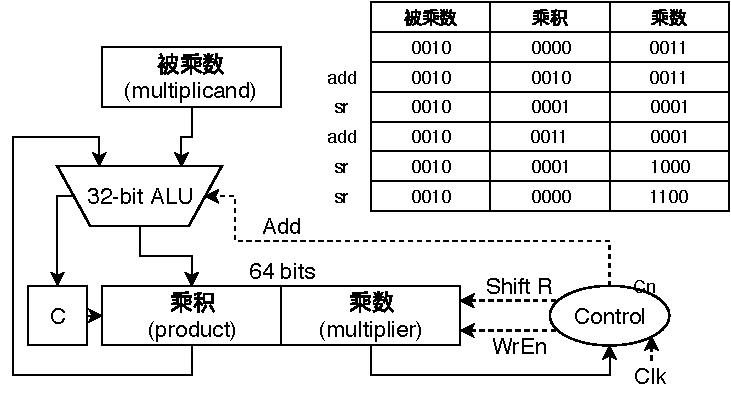
\includegraphics[width=0.6\linewidth]{fig/Arithmetic-Mulplication.pdf}
\end{figure}

\subsubsection{补码}
Booth乘法
\[[A\cdot B]_c=[A]_c\cdot([B]_c)_{\text{尾}}+[-A]_c\cdot B_0\]
\par 每一位的生成
\[\begin{aligned}
[P_{i+1}]_c&=2^{-1}\{[P_i]_c+(B_{n-i+1}-B_{n-i})[A]_c\}\qquad\mbox{当前乘数寄存器最后两位}\\
[P_{n+1}]_c&=[P_n]_c+(B_1-B_0)[A]_c
\end{aligned}\]
\par 根据(从左往右数)第$n$位和第$n+1$位的差,来决定进行什么操作
\begin{center}
\begin{tabular}{|c|c|c|}\hline
$(B_n,B_{n+1})$ & $[P_{i+1}]_c$ & op \\\hline
0 0 & $2^{-1}[P_i]_c$ & $>> 1$ \\\hline
0 1 & $2^{-1}([P_i]_c+[A]_c)$ & $+,>> 1$ \\\hline
1 0 & $2^{-1}([P_i]_c+[-A]_c)$ & $-,>> 1$ \\\hline
1 1 & $2^{-1}[P_i]_c$ & $>> 1$ \\\hline
\end{tabular}
\end{center}
\begin{itemize}
	\item 被乘数A和部分积P都取变形补码,乘数B取一位符号位,参与运算
	\item 乘数末尾增设附加位$B_{n+1}$,初始值为0
	\item 按补码移位规则(符号右移)
	\item 共$n+1$次移位(看乘数几位,不包符号),第$n+1$步部分积不移位
\end{itemize}
\begin{example}
定点小数$A=-0.011$,$B=0.101$,求$[A\cdot B]_c$
\end{example}
\begin{analysis}
\[\begin{aligned}
[A]_c&=11.101 \qquad &[-A]_c&=00.011\\
[B]_c&=0.101 \qquad &[P_0]_c&=00.000
\end{aligned}\]
\begin{center}
\begin{tabular}{|c|c|c|c|}\hline
& 被乘数 & 部分积 & 乘数\\\hline
初始化 & 11.101 & 00.000 & 0.101(0)\\\hline
加-A & 11.101 & 00.011 & 0.101(0)\\\hline
右移 & 11.101 & 00.001 & 10.10(1)\\\hline
加A & 11.101 & 11.110 & 10.10(1)\\\hline
右移(符号位)& 11.101 & 11.111 & 010.1(0)\\\hline
加-A & 11.101 & 00.010 & 010.1(0)\\\hline
右移 & 11.101 & 00.001 & 0010.(1)\\\hline
加A & 11.101 & 11.110 & 0010.(1)\\\hline
右移(仅乘数) & 11.101 & 11.110 & [0]001(0).\\\hline
\end{tabular}
\end{center}
\par 注意乘数首位为符号位,最后一步结合要忽略。
故$[A\cdot B]_c=1.110001$
\end{analysis}
\par * $(-1)\cdot(-1)$是\textbf{定点小数}补码乘法唯一移出的情况\\

\subsubsection{浮点数}
\begin{enumerate}
	\item 阶码相加减,判溢出
	\item 尾数相乘除
	\item 规格化,判溢出
	\item 舍入
	\item 确定符号位
\end{enumerate}

\subsubsection{运算器件}
伪加器(Carry Save Adder, CSA):将进位在本级加法器中保存,留待以后计算。
\par 三个$n$位数的和,需将伪加和$S_{p_i}$与左移一位的伪加进位$C_{p_i}$相加求得。
\par 柱形乘法器,采用多级CSA和一级普通并行加法器(CPA)构成

\subsection{除法}
\subsubsection{原码}
恢复余数除法:余数初始化为0,商初始化为被除数
\begin{itemize}
	\item 第一步除法A-B,之后余数-除数
	\item 若余数小于0,余数+除数,商0;否则商1
	\item 左移
\end{itemize}
\begin{figure}[H]
\centering
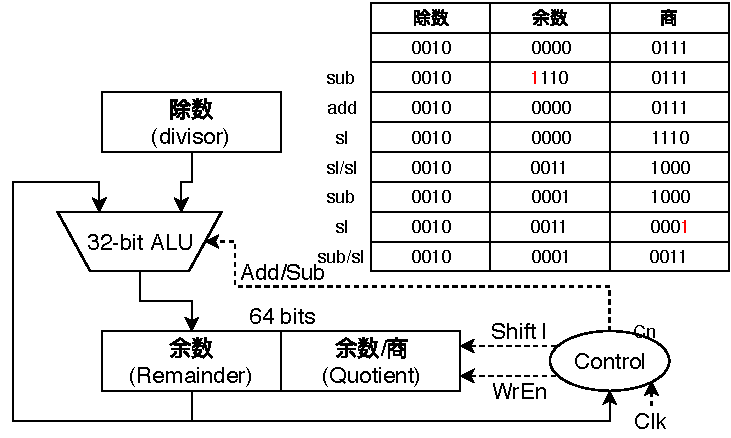
\includegraphics[width=0.6\linewidth]{fig/Arithmetic-Division.pdf}
\end{figure}
\par 加减交替法/不恢复余数法
\begin{itemize}
	\item 符号位单独处理
	\item 被除数(余数)设置双符号位,便于判断溢出
	\item $A-B$,余数为\textbf{正}/负,商为1/0,余数和商寄存器同步左移,左移后的余数\textbf{减}去/加上除数的绝对值得到新余数(本次余数为正,下步除法做减法;本次余数为负,下步除法做加法)
	\item 重复$n+1$步($n$位尾数,1位符号位)得到商的绝对值
	\item 最后一步余数\textbf{不}左移
	\item 若最后一步余数为负(假余数),则需加$|B|$得到正确的余数(只有最后一步需要恢复余数)
\end{itemize}

\subsubsection{补码}
Booth除法:先上商,后加减
\begin{itemize}
	\item 余数符号和除数符号上商,商左移
	\begin{itemize}
		\item 同号,商1,余数左移,减去除数
		\item 异号,商0,余数左移,加上除数
	\end{itemize}
	\item 最后一步上商,余数不变
	\item 商的符号取反
	\item 恢复余数和修正商
	\begin{itemize}
		\item 除法除尽时,余数寄存器全0
		\begin{itemize}
			\item 除数为正,商不必修正
			\item 除数为负,所得商加$2^{-n}$
		\end{itemize}
		\item 除法除不尽时
		\begin{itemize}
			\item 被除数与除数同号,且余数与除数异号,恢复余数:$[R_n]_c+[B]_c$
			\item 被除数与除数异号,且余数与除数同号,恢复余数:$[R_n]_c+[-B]_c$
			\item 商为证,商的反码与补码相同,不必修正
			\item 商为负,商的反码在末位加1,即加$2^{-n}$
		\end{itemize}
	\end{itemize}
\end{itemize}